\documentclass[t]{beamer}
\usepackage[english,spanish]{babel} 
\usepackage[utf8]{inputenc}         % Este paquete permite poner acentos directamente y e.es
\usepackage{multirow}
\usepackage{ffbeamer}
%\usepackage{beamerthemem}

%%% Si la presentación es en ingles, de lo contrartio comentar %%%
%\chooselanguage{english}

\title[FFT]{FFT }
%\author[Nombre corto]{Kunst, James}
\date{\today}
%\date{August 2017}


\begin{document}

\begin{frame}
\maketitle
\end{frame}

%%%%%%%%%%%%%%%%%%%%%%%%%%%%%%%%
\section[Outline]{}
%%%%%%%%%%%%%%%%%%%%%%%%%%%%%%%%
\begin{frame}
       \frametitle{Contenido}	
        \vspace*{0.5cm}
       %\framesubtitle{Tabla de contenidos}	
       \tiny{\tableofcontents}
\end{frame}
%%%%%%%%%%%%%%%%%%%%%%%%%%%%%%%%%


%\begin{frame}
%\frametitle{Photonic assisted ADC}	
%\vspace*{0.5cm}
% \begin{figure}[ht]
%    \centering
%  \includegraphics[height=0.35\paperheight]{image/padc1.png}
% \includegraphics[height=0.4\paperheight]{image/padc2.png}
%    \end{figure}
%\end{frame}


\begin{frame}
\frametitle{V1 y V2}	
\vspace*{0.5cm}
 \begin{figure}[ht]
    \centering
  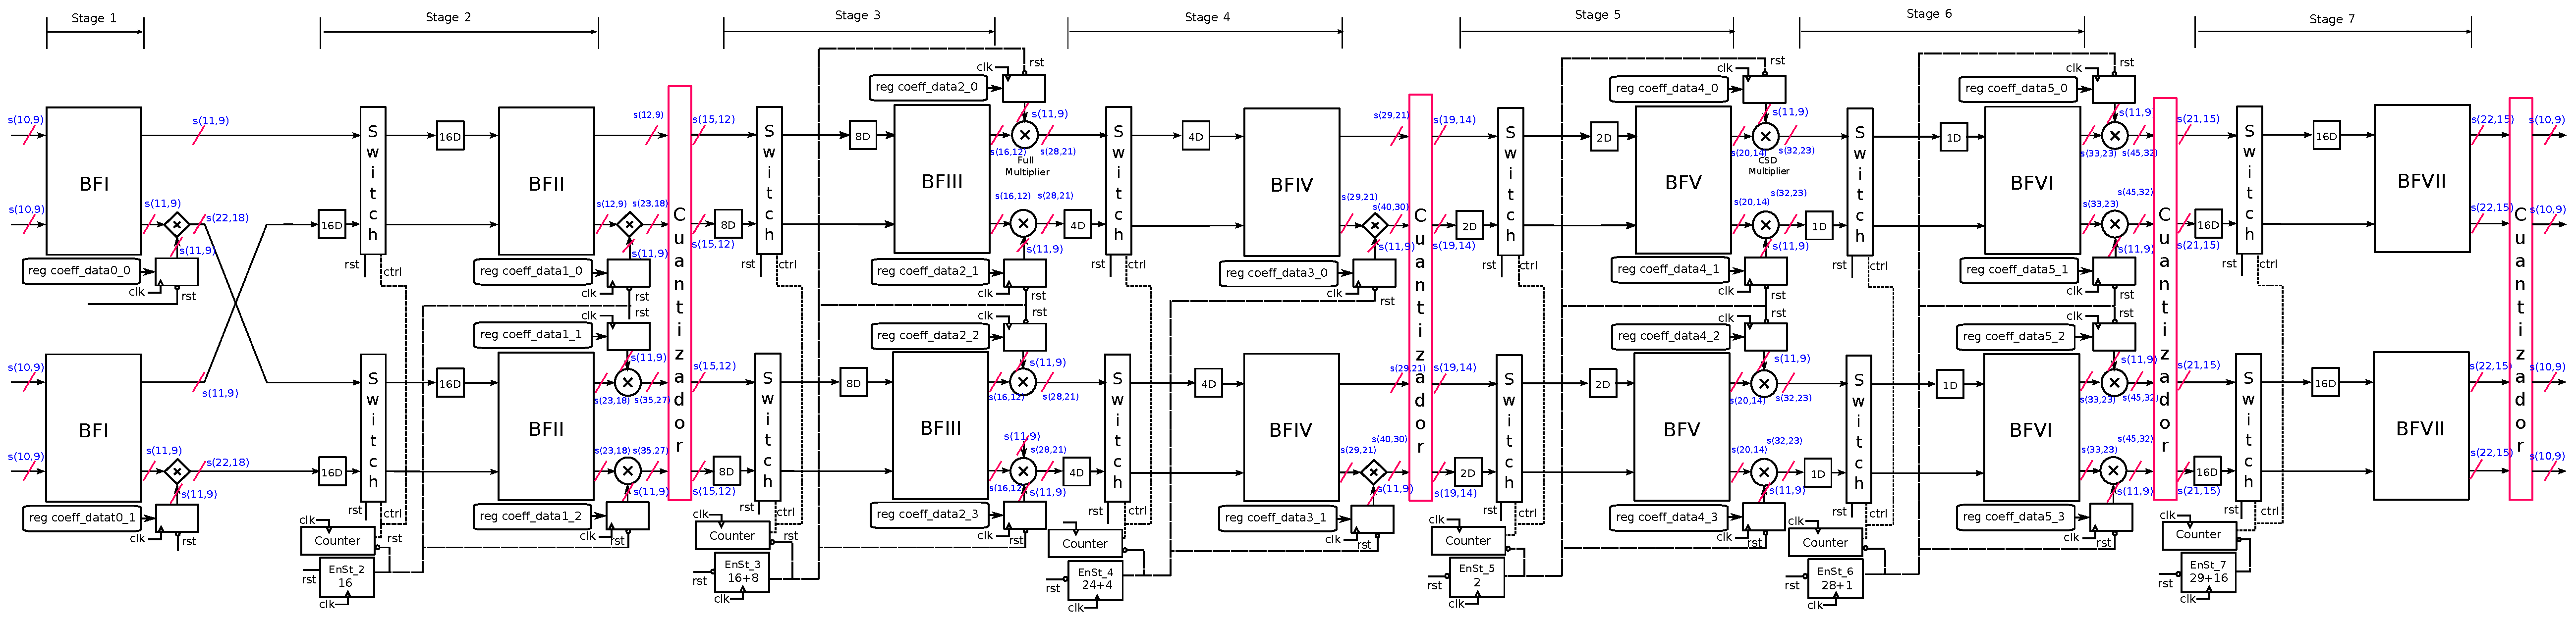
\includegraphics[height=0.28\paperheight]{image/V1_esquema.eps} \\
\hfill
  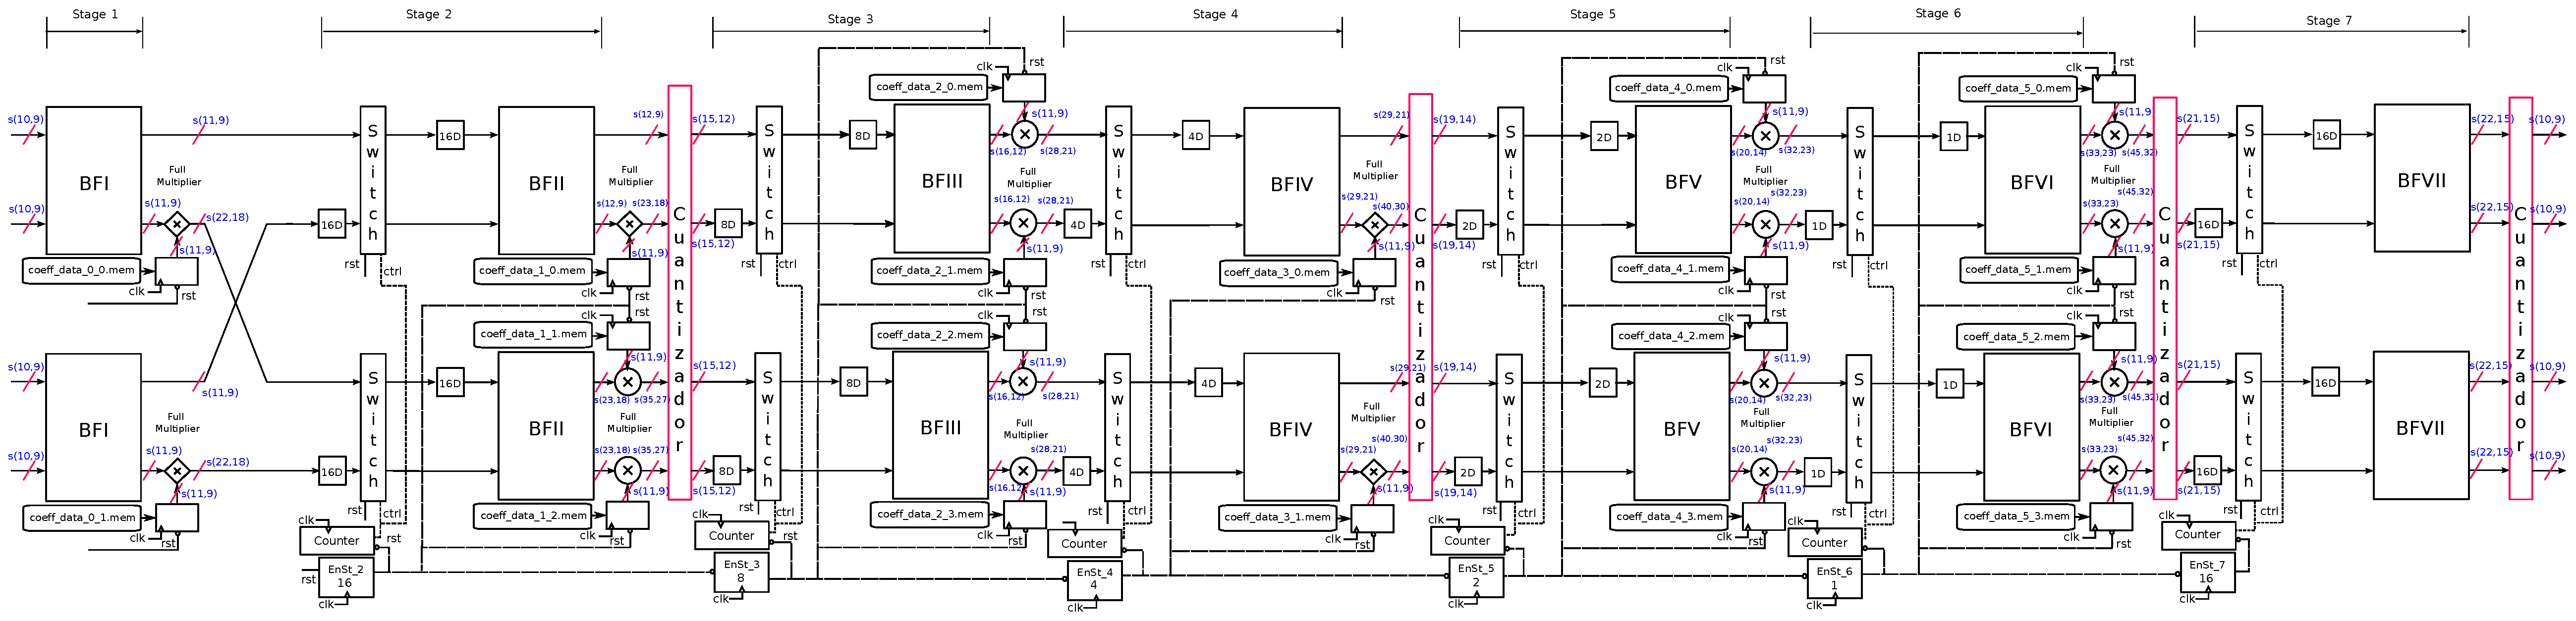
\includegraphics[height=0.28\paperheight]{image/V2_esquema.eps}
    \end{figure}
\end{frame}





\begin{frame}
\frametitle{V3  y V4}	
\vspace*{0.5cm}
 \begin{figure}[ht]
    \centering
  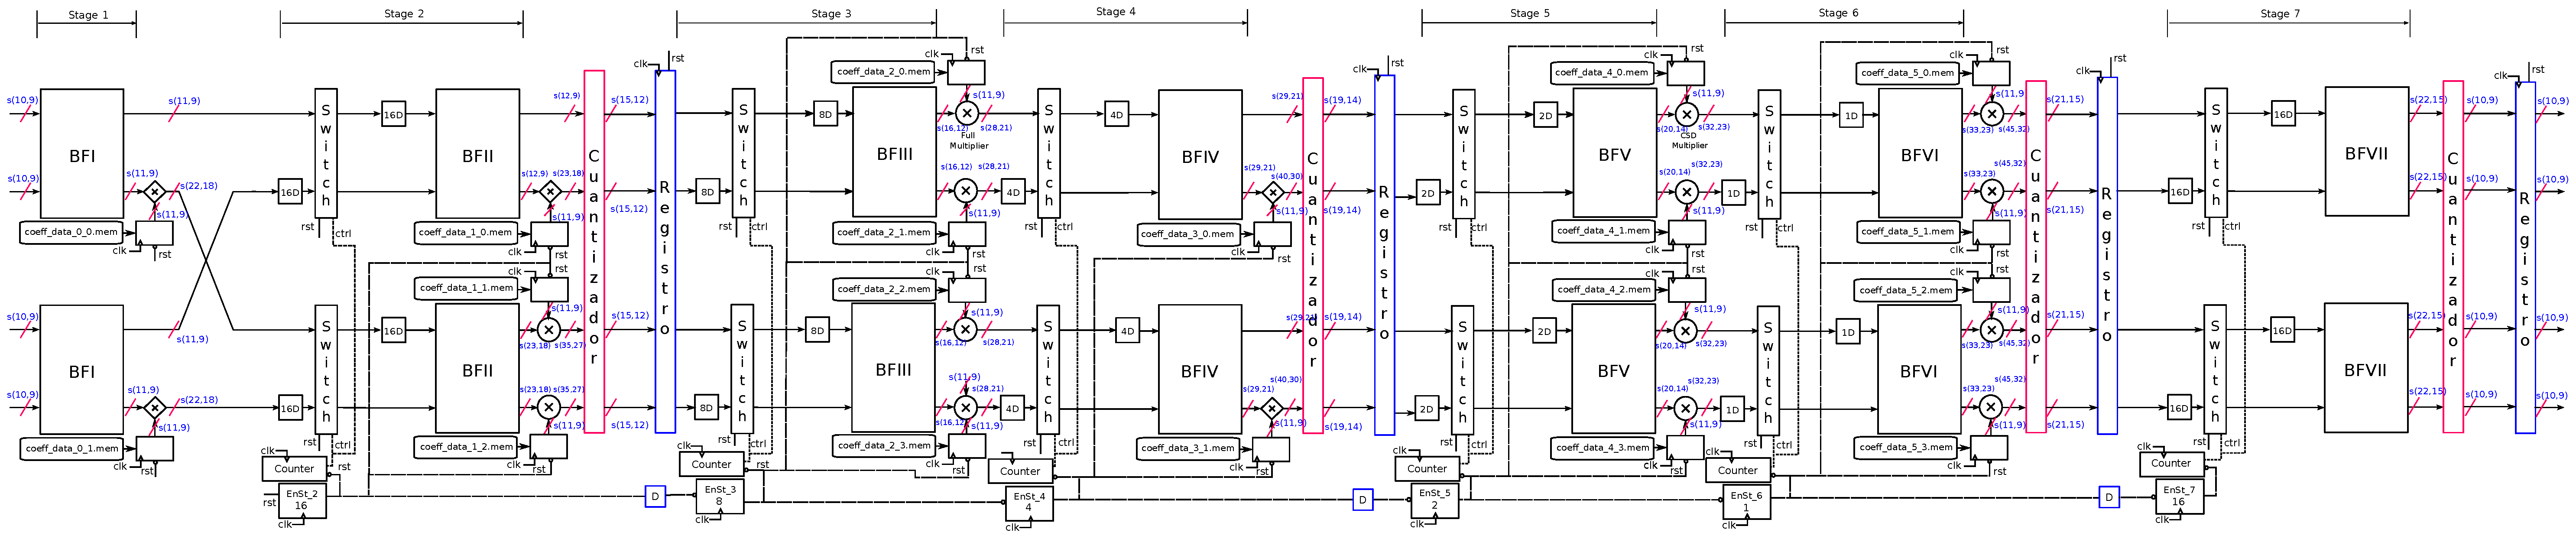
\includegraphics[height=0.25\paperheight]{image/V3_esquema.eps} \\
\hfill
  \includegraphics[height=0.25\paperheight]{image/V4_esquema.eps}
    \end{figure}
\end{frame}



\begin{frame}
\frametitle{V5 y V6}	
\vspace*{0.5cm}
 \begin{figure}[ht]
    \centering
  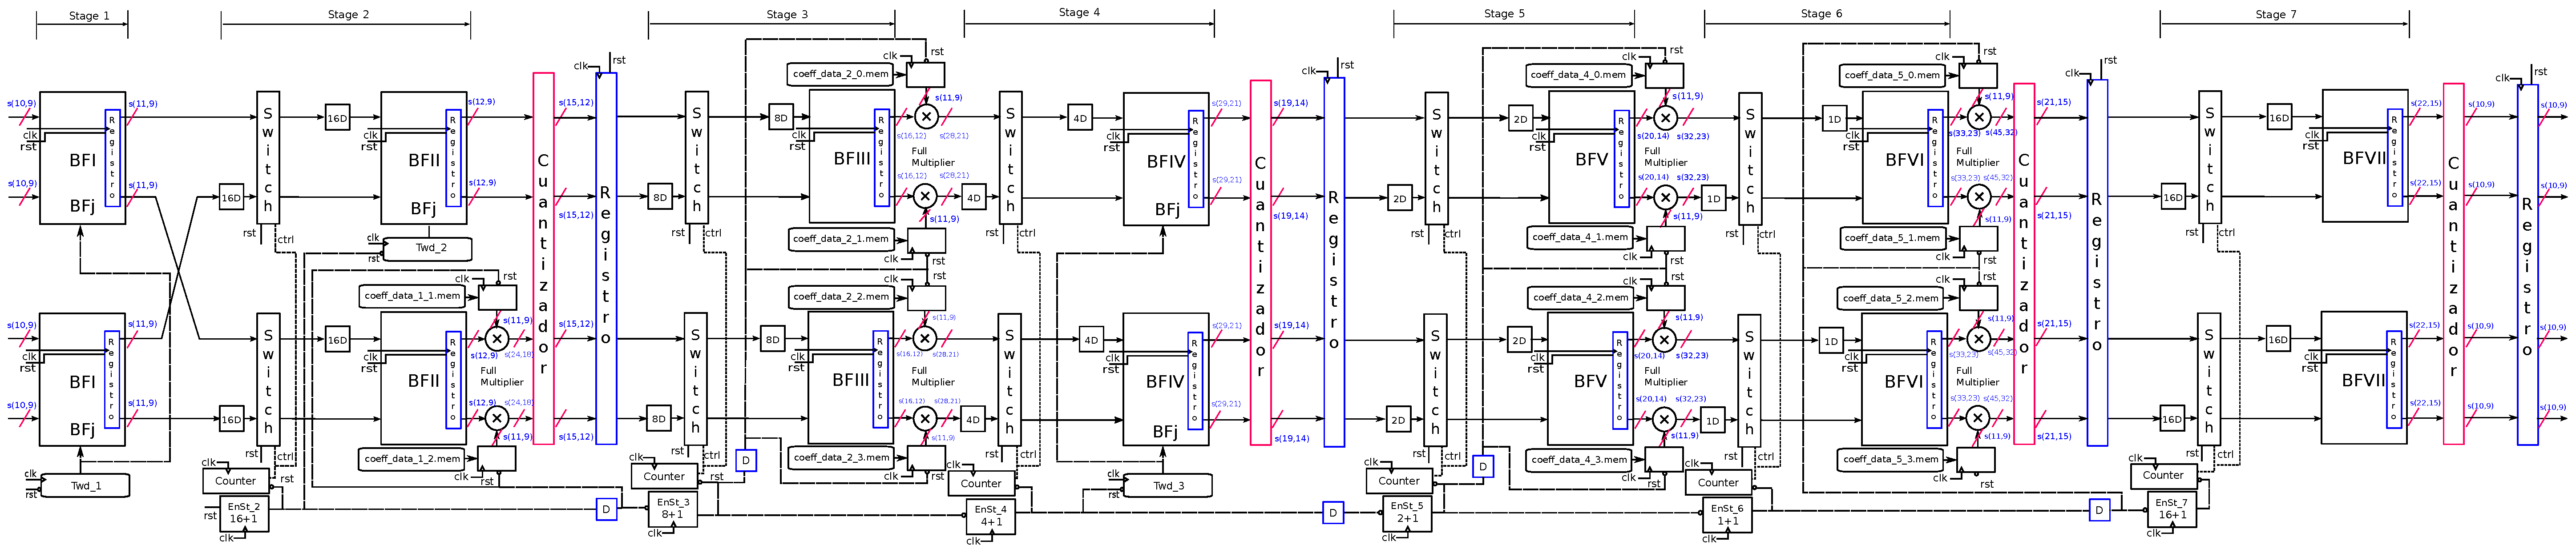
\includegraphics[height=0.25\paperheight]{image/V5_esquema.eps} \\
\hfill
  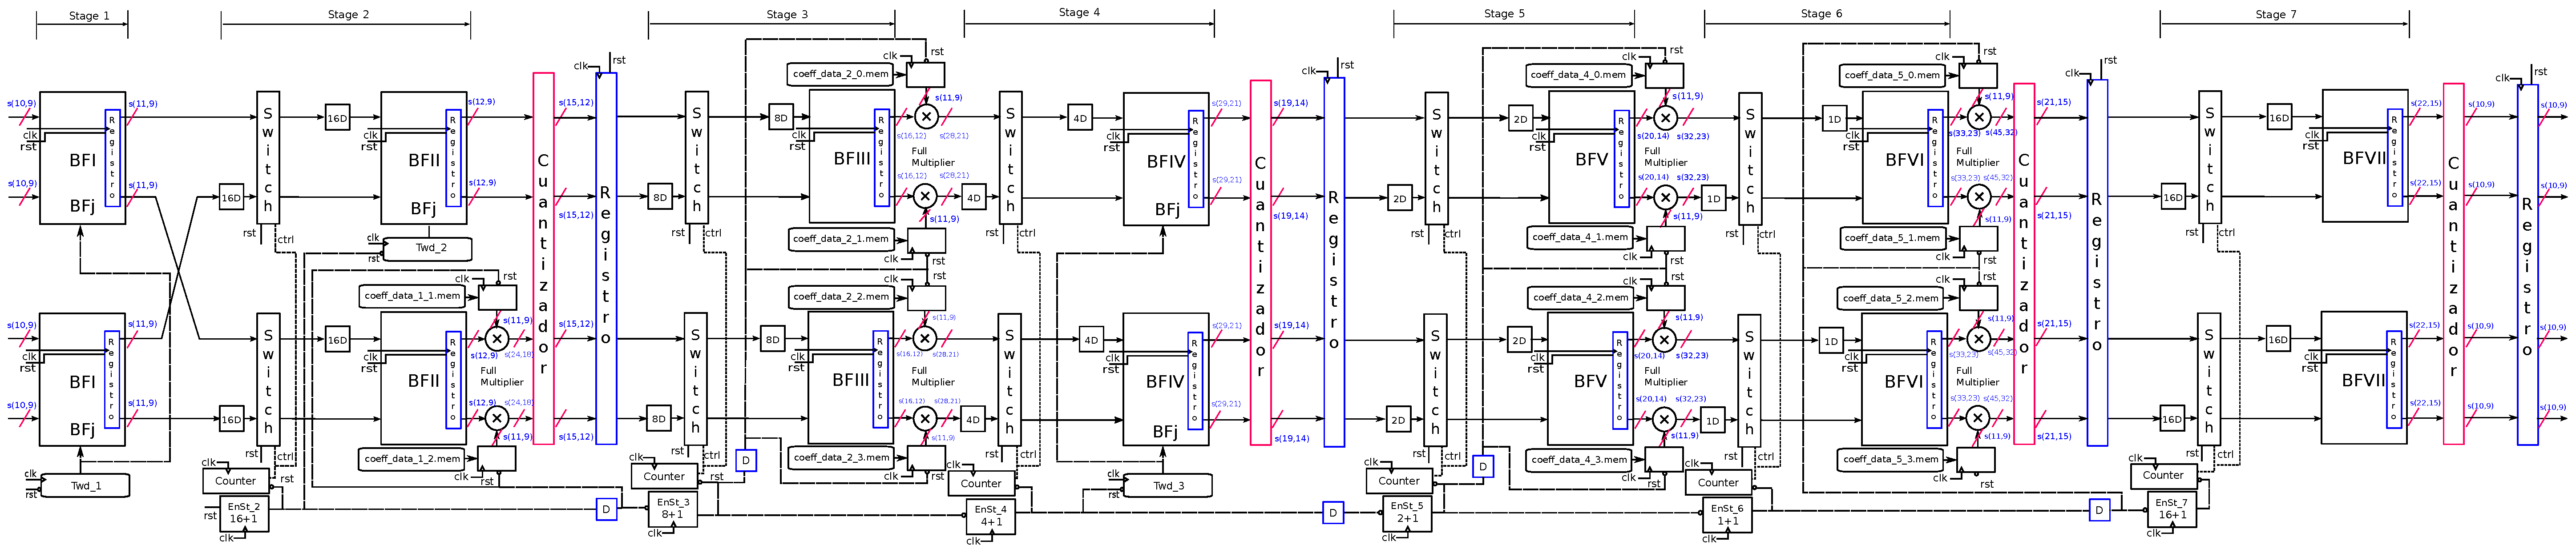
\includegraphics[height=0.25\paperheight]{image/V5_esquema.eps}
    \end{figure}
\end{frame}




%%%%%%%%%%%%%%%%%%%%%%%%%%%%%%%%-----END-----%%%%%%%%%%%%%%%%%%
\begin{frame}
 \frametitle{Fin}
   %\framesubtitle{The end}
\vspace*{2cm}
\centering
\begin{Huge}
    ¡Gracias!
\end{Huge}
\end{frame}
\end{document}


%%%%%%%%%%%%%%%%%%%%%%%%%%%%%%%%%%%%%%%%%%%%%%%%%%%%%%%%%%%%%%%%%%%%%%%%%%%%%%%%%%%%%%%%%%%%%%%%%%%%%%%%%%%%%%%%%%%%%%%%%%%%%%%%%%%%%%%%%%%%%%%%%%%%%%%%%%%%%%%%%%%%%%%%%%%%%%%%%%%%%%%%%%%%%










